%\vspace{-10pt}
\section{System Model}\label{sec:system_model}

Our system contains a task set \begin{math}\tau\end{math} of $n$ periodic or sporadic tasks (\begin{math}\tau_{1}\end{math}, \begin{math}\tau_{2}\end{math}, ..., \begin{math}\tau_{j}\end{math}, ..., \begin{math}\tau_{n}\end{math}) each scheduled on a single processor.  Each task \begin{math}\tau_{i}\end{math} is characterized by a tuple (\begin{math}C_{i}^{NP}\end{math}, \begin{math}D_{i}\end{math}, \begin{math}T_{i}\end{math}) where
%(\begin{math}\phi_{i}\end{math}, \begin{math}C_{i}^{NP}\end{math}, \begin{math}D_{i}\end{math}, \begin{math}T_{i}\end{math}, %\begin{math}J_{i}\end{math}, \begin{math}P_{i}\end{math}) where \begin{math}\phi_{i}\end{math} is the starting time (also known as the phase),
\begin{math}C_{i}^{NP}\end{math} is the non-preemptive worst case execution time, \begin{math}D_{i}\end{math} is the relative deadline, and 
%\begin{math}T_{i}\end{math} is the inter-arrival time or period, \begin{math}J_{i}\end{math} is the release %jitter and \begin{math}P_{i}\end{math} is
\begin{math}T_{i}\end{math} is the inter-arrival time or period.  
%and \begin{math}P_{i}\end{math} is the uniquely assigned static fixed priority.
Each task \begin{math}\tau_{i}\end{math} creates an infinite number of jobs, with the first job arriving at any time after system start time and subsequent jobs arriving no earlier than \begin{math}T_{i}\end{math} time units with a relative deadline \begin{math}D_{i}\end{math} \begin{math}\leq\end{math} \begin{math}T_{i}\end{math}.  The system utilizes a preemptive scheduler with each task/job containing \begin{math}N_{i}\end{math} number of basic blocks denoted (\begin{math}\delta_{i}^{0}\end{math}, \begin{math}\delta_{i}^{1}\end{math}, \begin{math}\delta_{i}^{2}\end{math}, ..., \begin{math}\delta_{i}^{N_{i}}\end{math}) with the total number of basic blocks given by N = \begin{math}\Sigma_{i}\end{math}\begin{math}N_{i}\end{math}. A dummy basic block \begin{math}\delta_{i}^{0}\end{math} with zero WCET is added at the beginning of each task to capture the preemption that occurs prior to task execution.  In our sequential model, a basic block is a set of one or more instructions that execute non-preemptively.  Basic blocks are essentially the vertices $V$ of a control flow graph (CFG) connected in a sequence by edges $E$ representing the execution sequence of one or more job instructions. Figure~\ref{fig:system_model} shown below illustrates the sequential basic block connection structure.
%denoted as \begin{math}\delta_{i}^{b}\end{math} using our convention.
\vspace{-5pt}
\begin{figure}[h!]
\begin{center}
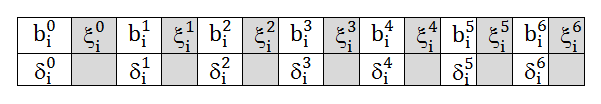
\includegraphics[width=0.5\textwidth]{system_model.png}
\caption{System Model.}
\label{fig:system_model}
\end{center}
\vspace{-10pt}
\end{figure}
\noindent
Preemptions are permitted at basic block boundaries.  We introduce the basic block notation \begin{math}\delta_{i}^{j}\end{math} where $i$ is the task identifier and $j$ is the basic block identifier. We introduce the the non-preemptive basic block execution time notation \begin{math}b_{i}^{j}\end{math} where $i$ is the task identifier and $j$ is the basic block identifier, hence using this convention we have
\begin{equation}\label{eqn:c-np2}
    C_{i}^{NP} = \Sigma_{j}\ b_{i}^{j}.
\end{equation}
\noindent
%The task release jitter \begin{math}J_{i}\end{math} is defined as the maximum time between the task arriving for execution and it being released to a %state of being ready to execute.  In our work, we assume the release jitter \begin{math}J_{i}\end{math} = 0.
The processor utilization \begin{math}U_{i}\end{math} of task \begin{math}\tau_{i}\end{math} is given by
\begin{equation}\label{eqn:u-task}
    U_{i} = C_{i}^{NP}/T_{i}.
\end{equation}
\noindent
The maximum blocking time $Q_i$ is the maximum duration that a task $\tau_i$ can be blocked due to non-preemptive execution of a lower priority task. The preemption cost as a function of the current
and next preemption points is given by the variable $\xi_{i}$ as discussed in section~\ref{sec:schedulability_analysis}.  
%Blocking time \begin{math}\beta_{i}\end{math} is the duration of time which task \begin{math}\tau_{i}\end{math} %is unable to execute due to a lower priority task that either executes non-preemptively or holds a resource %that is shared with task \begin{math}\tau_{i}\end{math} or any other task of equal or higher priority.
%In our work, we remove the restriction of a linear basic block structure thereby permitting an arbitrarily %connected basic block structure.
%A direct-mapped cache is assumed. 
Tasks may be preempted by multiple higher-priority tasks identified by the variable $k$ comprising the set of higher priority tasks for task \begin{math}\tau_{i}\end{math}. For example for both Deadline-Monotonic (DM) and Earliest-Deadline-First (EDF) scheduling, the set of higher priority tasks is represented by:
%For fixed priority (FP) scheduling we have:
%\begin{equation}\label{eqn:fp-hp-tasks}
%    k \in hp(i) = \{k | P_{k} > P_{i}\}.
%\end{equation}
%\noindent
%For Earliest Deadline First (EDF) scheduling, we have:
\begin{equation}\label{eqn:edf-hp-tasks}
    k \in hp(i) = \{k | D_{k} < D_{i}\}.
\end{equation}
\noindent
The set of higher priority tasks needs to be filtered by tasks that may preempt during the execution window of task \begin{math}\tau_{i}\end{math}.  The number of times task \begin{math}\tau_{k}\end{math} can preempt task \begin{math}\tau_{i}\end{math} during task \begin{math}\tau_{i}\end{math}'s execution is given by the term
\begin{equation}\label{eqn:num-preemptions}
    N_{p}(\tau_{i},\tau_{k})=\lceil(C_{i}/T_{k})\rceil \geq 1.
%    N_{p}(\tau_{i},\tau_{k})=\lceil(C_{i} + J_{k})/T_{k})\rceil \geq 1.
\end{equation}
\noindent
where $k$ is the index of the preempting task \begin{math}\tau_{k}\end{math} and $i$ is the index of the preempted task \begin{math}\tau_{i}\end{math}.  In a limited preemption approach, each task is permitted to execute non-preemptively for a maximum amount of time denoted by \begin{math}Q_{i}\end{math}.  Previous research on limited preemption scheduling (e.g., Baruah~\cite{baruah:05}) has used the above information to determine the value of $Q_i$ for each task.  Therefore, we assume that $Q_i$ is provided by such an approach.
%
%\begin{center}
%  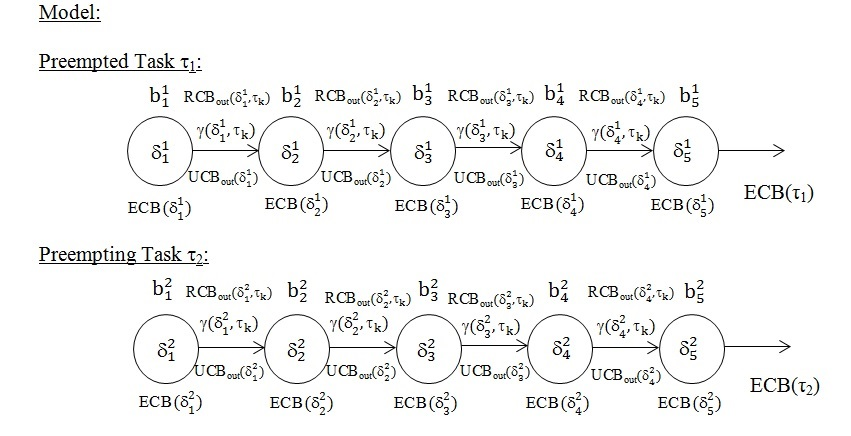
\includegraphics[width=\linewidth, height=.25\textheight]{system_model.jpg}
%\end{center}

